\section{Como correr o programa}

Para correr o programa desenvolvido temos várias opções. Para saber qual a sintaxe pela qual o programa se rege deve-se chamar o programa seguido do argumento -h:
\begin{itemize}
	\item perl signpdf\_cli.pl -h
\end{itemize} 
\hfill\newline
O programa requer sempre 3 inputs obrigatórios:
\begin{itemize}
	\item Número de telemóvel do utilizador
	\item Pin da chave móvel digital
	\item Nome do pdf a assinar
\end{itemize}
\hfill\newline
Adicionalmente o programa permite ao utilizador fornecer 2 inputs extra \textit{Output file} e \textit{Datetime} que são respetivamente o nome a ser atribuido ao pdf assinado e a data a usar para assinar o mesmo, podendo o utilizador escolher fornecer apenas o primeiro, apenas o segundo ou ambos.\newline
Assim, apresentam-se em seguida as várias combinações disponíveis para a utilização da app:
\begin{enumerate}
	\item perl signpdf\_cli.pl -u '+351 XXXXXXXXX' -p X{4-8} -infile 'nome do ficheiro'.pdf
	\item perl signpdf\_cli.pl -u '+351 XXXXXXXXX' -p X{4-8} -infile 'nome do ficheiro'.pdf - outputfile 'nome do ficheiro'.pdf
	\item perl signpdf\_cli.pl -u '+351 XXXXXXXXX' -p X{4-8} -infile 'nome do ficheiro'.pdf -datetime YYYY-MM-DDTHH:MM:SS.SSSSSS
	\item perl signpdf\_cli.pl -u '+351 XXXXXXXXX' -p X{4-8} -infile 'nome do ficheiro'.pdf - outputfile 'nome do ficheiro'.pdf -datetime YYYY-MM-DDTHH:MM:SS.SSSSSS
\end{enumerate}


Caso corra a aplicação como um utilizador regular (sem debug) o resultado esperado é o seguinte:
\begin{figure}[H]

  \centering
  \captionsetup{justification=centering}

  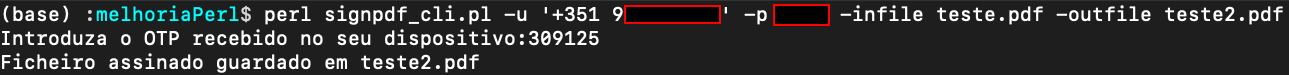
\includegraphics[scale = 0.25]{resultado1.png}
  
  \caption {Resultado de correr o programa sem o modo debug}

\end{figure}


 Caso corra a aplicação como um utilizador regular o resultado esperado é o seguinte:

\begin{figure}[H]

  \centering
  \captionsetup{justification=centering}

  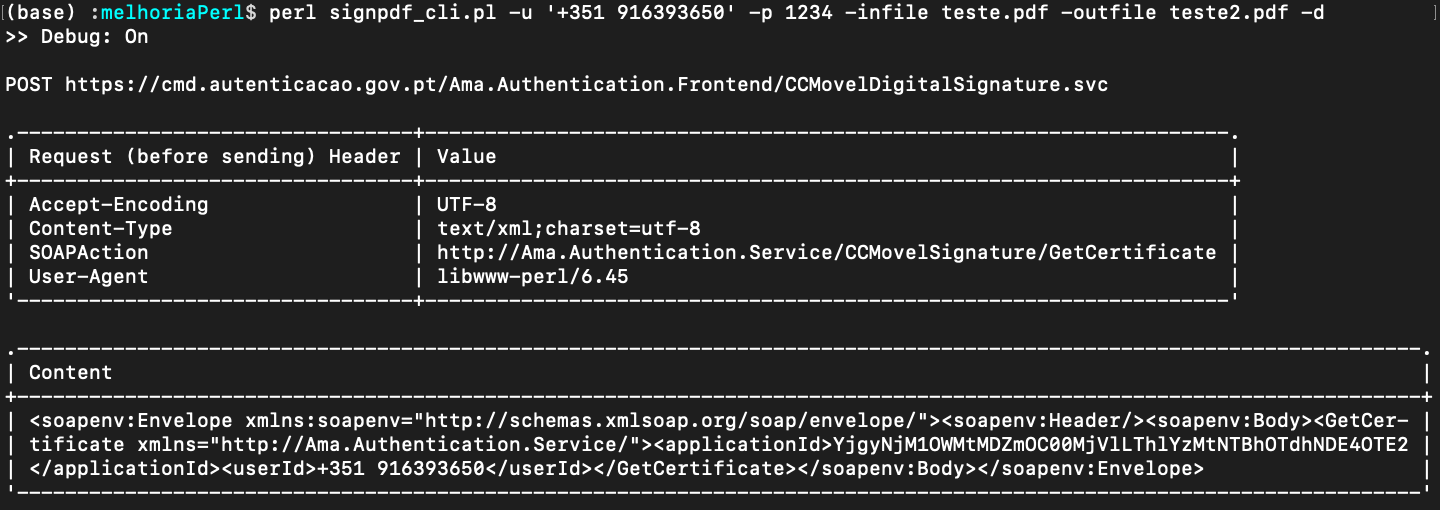
\includegraphics[scale = 0.25]{resultado2.png}
  
  \caption {Resultado de correr o programa com o modo debug}

\end{figure}







